\documentclass[11pt,border=5pt]{standalone}
\usepackage{fontspec}
\setmainfont{cmunrm.otf}[BoldFont=cmunbx.otf,ItalicFont=cmunti.otf,BoldItalicFont=cmunbi.otf]
\usepackage{amsmath}
\usepackage{unicode-math}
\setmathfont{NewCMMath-Regular.otf}
\usepackage{tikz}
\usetikzlibrary{arrows.meta,patterns,angles,quotes}
\begin{document}
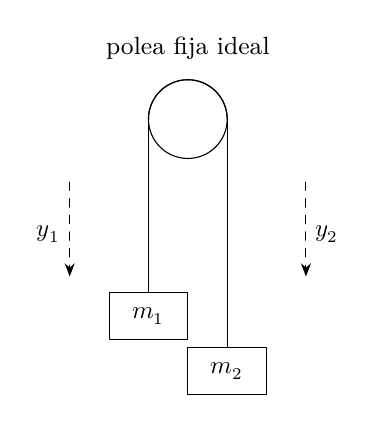
\begin{tikzpicture}[>=Stealth,font=\small,line cap=round,line join=round]
\draw (0,1.5) circle (.5);\draw (-.5,1.5)--(-.5,-.8);\draw (.5,1.5)--(.5,-1.5);\draw (-.5,1.5) arc (180:0:.5);
\draw[fill=white] (-1.0,-1.3) rectangle (0.0,-0.7);
\node at (-0.5,-1) {$m_1$};
\draw[fill=white] (0.0,-2.0) rectangle (1.0,-1.4);
\node at (0.5,-1.7) {$m_2$};
\draw[->,thin,dashed] (-1.5,0.7) -- (-1.5,-0.5) node[pos=0.55,left] {$y_1$};
\draw[->,thin,dashed] (1.5,0.7) -- (1.5,-0.5) node[pos=0.55,right] {$y_2$};
\node at (0,2.4) {polea fija ideal};

\end{tikzpicture}
\end{document}
